%%%%%%%%%%%%%%%%%%%%%%%%%%%%%%%%%%%%%%%%%
% Programming/Coding Assignment
% LaTeX Template
%
% This template has been downloaded from:
% http://www.latextemplates.com
%
% Original author:
% Ted Pavlic (http://www.tedpavlic.com)
%
% Note:
% The \lipsum[#] commands throughout this template generate dummy text
% to fill the template out. These commands should all be removed when 
% writing assignment content.
%
% This template uses a Perl script as an example snippet of code, most other
% languages are also usable. Configure them in the "CODE INCLUSION 
% CONFIGURATION" section.
%
%%%%%%%%%%%%%%%%%%%%%%%%%%%%%%%%%%%%%%%%%

%----------------------------------------------------------------------------------------
%	PACKAGES AND OTHER DOCUMENT CONFIGURATIONS
%----------------------------------------------------------------------------------------

\documentclass{article}

\usepackage{fancyhdr} % Required for custom headers
\usepackage{lastpage} % Required to determine the last page for the footer
\usepackage{extramarks} % Required for headers and footers
\usepackage[usenames,dvipsnames]{xcolor} % Required for custom colors
\usepackage{graphicx} % Required to insert images
\usepackage{wrapfig} % Wraping text around images
\usepackage{listings} % Required for insertion of code
\usepackage{courier} % Required for the courier font
\usepackage{lipsum} % Used for inserting dummy 'Lorem ipsum' text into the template
\usepackage[utf8]{inputenc} % UTF8 for öäöüéè...
\usepackage[T1]{fontenc} % Wordsplitting
\usepackage[many]{tcolorbox} % Textbox
\usepackage{xargs} % For more then one optional Argument
%\usepackage{ngerman} % German Captures
\usepackage[autostyle=true,german=quotes]{csquotes} % Anführungszeichen nach Deutschem Norm
\usepackage[sort]{acro} %Fussnote mit Verzeichnis
\usepackage{pgfgantt}
\usepackage{rotating}
\usepackage{float}
\usepackage{titlesec}
\usepackage{hyperref}
\usepackage[useregional]{datetime2}
\usepackage{makecell}
\usepackage{tabularx}
\usepackage{csvsimple}
\usepackage{longtable}
\usepackage{uarial}
\usepackage{upquote}
\usepackage{enumitem}
\usepackage{nameref}
\usepackage{pgfplots}
\usepackage{subcaption}
\usepackage{url}
\usepackage{microtype}
\usepackage{multimedia}
\usepackage{array}
\usepackage{pgfplotstable}
\usepackage{eso-pic} % Background image
\usepackage{apacite}
\pgfplotsset{compat=1.16}
\renewcommand{\familydefault}{\sfdefault}


% Margins
\topmargin=-0.45in
\evensidemargin=0in
\oddsidemargin=0in
\textwidth=6.5in %6.5in
\textheight=9.0in
\headsep=0.25in

\linespread{1.1} % Line spacing
\setlist[1]{nolistsep}

%\renewcommand{\familydefault}{\sfdefault}

% Set up the header and footer
\pagestyle{fancy}
\lhead{Stefan Jampen \& Damian Moser} % Top left header
\chead{IDPA} % Top center head
\rhead{\nouppercase{\rightmark}} % Top right header \firstxmark
\lfoot{\lastxmark} % Bottom left footer
% Neues Logo suchen
\cfoot{}
% \cfoot{\vspace*{-1.88\baselineskip}
\includegraphics[scale=0.33]{abacuslogo}\vspace*{1.88\baselineskip}} % Bottom center footer
\rfoot{Side\ \thepage\ of\ \protect\pageref{LastPage}} % Bottom right footer
\renewcommand\headrulewidth{0.4pt} % Size of the header rule
\renewcommand\footrulewidth{0.4pt} % Size of the footer rule

\setlength\parindent{0pt} % Removes all indentation from paragraphs
%\setcounter{tocdepth}{2}
%\setcounter{secnumdepth}{0} % Removes default section numbers
\setcounter{secnumdepth}{4}
\setcounter{tocdepth}{4}

%----------------------------------------------------------------------------------------
%	CODE INCLUSION CONFIGURATION
%----------------------------------------------------------------------------------------

\lstset{frame=single, % Single frame around code
		inputencoding={utf8},
		extendedchars=false,  
        basicstyle=\small\ttfamily, % Use small true type font
        keywordstyle=[1]\color{Blue}\bf, % Perl functions bold and blue
        keywordstyle=[2]\color{Purple}, % Perl function arguments purple
        keywordstyle=[3]\color{Blue}\underbar, % Custom functions underlined and blue
        identifierstyle=, % Nothing special about identifiers                                         
        commentstyle=\usefont{T1}{pcr}{m}{sl}\color{Green}\small, % Comments small dark green courier font
        stringstyle=\color{Purple}, % Strings are purple
        showstringspaces=false, % Don't put marks in string spaces
        tabsize=4, % 5 spaces per tab
        %
        % Put standard Perl functions not included in the default language here
        %morekeywords={rand},
        %
        % Put Perl function parameters here
        %morekeywords=[2]{on, off, interp},
        %
        % Put user defined functions here
        %morekeywords=[3]{test},
       	%
        morecomment=[l][\color{Blue}]{...}, % Line continuation (...) like blue comment
        numbers=left, % Line numbers on left
        firstnumber=1, % Line numbers start with line 1
        numberstyle=\tiny\color{Blue}, % Line numbers are blue and small
        stepnumber=5, % Line numbers go in steps of 5
        captionpos=b% Position of the Caption
}


%----------------------------------------------------------------------------------------
%	DOCUMENT STRUCTURE COMMANDS
%	Skip this unless you know what you're doing
%----------------------------------------------------------------------------------------


%----------------------------------------------------------------------------------------
%	NAME AND CLASS SECTION
%----------------------------------------------------------------------------------------

\renewcommand{\Nameref}[1]{`\nameref{#1}' auf der Seite~\pageref{#1}}
\titleformat{\paragraph}
{\normalfont\normalsize\bfseries}{\theparagraph}{1em}{}
\titlespacing*{\paragraph}
{0pt}{3.25ex plus 1ex minus .2ex}{1.5ex plus .2ex}
%----------------------------------------------------------------------------------------
%	TITLE PAGE
%----------------------------------------------------------------------------------------
\newcommand\BackgroundPic{
\put(0,-100){%
\parbox[b][\textheight]{\textwidth}{%
\vfill
\centering

\includegraphics[width=\textwidth,height=\textheight,%
keepaspectratio]{background2.jpg}%
\vfill
}}}
\newcommand{\HRule}[1]{\rule{\linewidth}{#1}}
\title{ \normalsize \textsc{Documentation\\IDPA}
		\\ [2.0cm]
		\HRule{2pt} \\
		\LARGE \textbf{\uppercase{Target oriented application of a SLAP algorithm for Ultimate Tic Tac Toe}}
		\HRule{2pt} \\ [0.5cm]
		\normalsize  \vspace*{5\baselineskip}}

\date{}

\author{
		Stefan Jampen \\ 
        	Damian Moser \\
		Guided By - Alejandro González and Barbara Becher \\
		Gewerbliche Berufsschule St.Gallen}



%\title{
%\LARGE{Dokumentation}
%}
%
%%\author{\textbf{\hmwkAuthorName}}
%\author{}
%\date{} % Insert date here if you want it to appear below your name

%----------------------------------------------------------------------------------------

\graphicspath{{./img/}}
\newcommand\todo[1]{\textcolor{red}{\\\\//TODO #1\\}}

%\newcolumntype{L}[1]{>{\raggedright\let\newline\\\arraybackslash\hspace{0}}{#1}}
%\newcolumntype{C}[1]{>{\centering\let\newline\\\arraybackslash\hspace{0}}m{#1}}
%\newcolumntype{R}[1]{>{\raggedleft\let\newline\\\arraybackslash\hspace{.2in}}m{#1}}
\newcolumntype{R}{>{\raggedleft\arraybackslash}p{.2in}}


\abovecaptionskip=3pt % above caption
\belowcaptionskip=\baselineskip % below caption
\newenvironment{fixedpic}{
\break
\begin{minipage}{\linewidth}
\abovecaptionskip=3pt % above caption
\belowcaptionskip=\baselineskip % below caption
\centering
}{
\end{minipage}
}


\acsetup{first-style=short}
\acsetup{first-style=footnote}

\DeclareAcronym{UTTT}{
	short=UTTT,
	long=Ultimate Tic-Tac-Toe,
}

\DeclareAcronym{organism}{
	short=organism,
	short-plural-form=organisms,
	long=The organism contains the DNA and is part of a generation.,
}

\DeclareAcronym{generation}{
	short=generation,
	short-plural-form=generations,
	long=A generation contains several organisms,
}

\DeclareAcronym{era}{
	short=era,
	long=An era is a set of generations,
}

\DeclareAcronym{SLAP}{
	short=SLAP,
	long=Self Learning Alpha Beta Pruning,
}

\DeclareAcronym{SL}{
	short=SL,
	long=Self Learning,
}

\DeclareAcronym{ABP}{
	short=ABP,
	long=Alpha Beta Pruning,
}

\DeclareAcronym{DNA}{
	short=DNA,
	long={A mutable factor, which dictates the importance of a condition},
}

\DeclareAcronym{condition}{
	short=condition,
	short-plural-form=conditions,
	long={In our context, a condition is a heuristic parameter. In our heuristic, exactly five 			conditions exist},
}

\DeclareAcronym{heuristic}{
	short=heuristic,
	long={With the heuristic, we evaluate a meaningful number, which corresponds with an 			arbitrary game state},
}

\DeclareAcronym{thread}{
	short=thread,
	long={A thread is a single unit of execution within a process. Normally, one thread at a time is executed by one core of a processor. },
}

\DeclareAcronym{UI}{
	short=UI,
	long=User Interface,
}

\DeclareAcronym{responsive}{
	short=responsive,
	long=Erklärung,
}

\DeclareAcronym{BMS}{
	short=BMS,
	long=Berufs Mittel Schule,
}

\DeclareAcronym{IDPA}{
	short=IDPA,
	long=InterDisziplinäre Projekt Arbeit,
}

\DeclareAcronym{game state}{
	short=game state,
	long={A game state is any possible configuration on the UTTT field.},
}
 % Configure wortdefinitionen
\definecolor{abablack}{HTML}{282828}
\definecolor{abared}{HTML}{de323C}
\definecolor{abablue}{HTML}{1677cb}
\definecolor{abaorange}{HTML}{ffa539}
\definecolor{abagray}{HTML}{5b5b5b}

\pgfplotscreateplotcyclelist{abacus}{%
abablack,every mark/.append style={fill=abablack},mark=triangle*\\%
abared,every mark/.append style={fill=abared},mark=*\\%
abablue!60!black,every mark/.append style={fill=abablue},mark=pentagon*\\%
abaorange,every mark/.append style={fill=abaorange},mark=square*\\%
abagray,every mark/.append style={fill=abagray},mark=diamond*\\%
}
\pgfplotscreateplotcyclelist{abacusbar}{%
abablack,fill=abablack!70!white,mark=none\\%
abared,fill=abared!70!white,mark=none\\%
abablue,fill=abablue!70!white,mark=none\\%
abaorange,fill=abaorange!70!white,mark=none\\%
abagray,fill=abagray!70!white,mark=none\\%
}

\pgfplotscreateplotcyclelist{abacus235}{%
abared,every mark/.append style={fill=abared},mark=*\\%
abablue!60!black,every mark/.append style={fill=abablue},mark=pentagon*\\%
abagray,every mark/.append style={fill=abagray},mark=diamond*\\%
}
\pgfplotscreateplotcyclelist{abacusbar235}{%
abared,fill=abared!70!white,mark=none\\%
abablue,fill=abablue!70!white,mark=none\\%
abagray,fill=abagray!70!white,mark=none\\%
}



%\pgfplotscreateplotcyclelist{abacusbar}{%
%abablack,fill=abablack!30!white,mark=none\\%
%abared,fill=abared!30!white,mark=none\\%
%abablue,fill=abablue!30!white,mark=none\\%
%abaorange,fill=abaorange!30!white,mark=none\\%
%abagray,fill=abagray!30!white,mark=none\\%
%}
\newenvironment{dnadiagram}{
\begin{tikzpicture}
\begin{axis}[
width=8.5cm,
ylabel=Value DNA,
xlabel=Condition,
legend style={at={(0.5,1.05)},
anchor=south,legend columns=-1},
%xtick={0,1,2,3,4,5,6},
xticklabels={1, 2, 3, 4, 5},
xticklabel={\pgfmathprintnumber[assume math mode=true]{\tick}},
yticklabel={\pgfmathprintnumber[assume math mode=true]{\tick}},
%x tick label style={rotate=90},
%cycle list name=abacus235,
]
}{
\end{axis}
\end{tikzpicture}
}


\begin{document}
\AddToShipoutPicture*{\BackgroundPic}
\maketitle
\thispagestyle{empty}

%----------------------------------------------------------------------------------------
%	TABLE OF CONTENTS
%----------------------------------------------------------------------------------------

%\setcounter{tocdepth}{1} % Uncomment this line if you don't want subsections listed in the ToC

\newpage
\tableofcontents
\newpage

%----------------------------------------------------------------------------------------
%	PROBLEM 1
%----------------------------------------------------------------------------------------

% To have just one problem per page, simply put a \clearpage after each problem

\section{Introduction}
%introduction of the topic
Algorithms are everywhere. They are a part of our everyday lives without even realizing it. They can be found in general mathematics, or in practical applications such as  computers or smartphones. But what exactly is an algorithm? According to the Oxford Dictionary an algorithm is generally speaken "a process or set of rules to be followed in calculations or other problem-solving operations, especially by a computer" \cite{web:oxforddictionaries2018}.
In our apprenticeship, we both have a lot to do with algorithms. Damian works as a software engineer, where he writes most of the time software. Stefan is an electronics engineer and his specialisation in the fourth year of education is also software. According to that, we both have a pretty good idea of what algorithms are and what they do. We found out, that each of us is fascinated by the concepts and possibilities algorithmic structures provide. So we came up with the idea, to implement an algorithm by ourselves. \\

%goals
We set the goal, to program an algorithm, that can play the game \acl{UTTT} (\ac{UTTT}). \ac{UTTT} is a more complex and strategic version of the ordinary Tic-Tac-Toe. 
Our approach to solve that problem is a so called \acl {SLAP}  algorithm, also known as \ac{SLAP} Algorithm. It's a combination of the already existing \acl{ABP} algorithm (\ac{ABP}) combined with an own made up extension which is, as the name suggests, self learning. We want to analyse the learning process of the algorithm in more detail and evaluate whether there is really an improvement. This will be the mathematical part of our work.
To experience our algorithm in action, we also wanted to create a website where everybody can play the game against our \ac{SLAP} Algorithm.
Another intention of our project is to bring the seemingly complex subject in an easy understandable form to the interested reader. We aim to resume our approach of the solution in a comprehensible way. We want to give the reader an insight and a deeper understanding of algorithms, how they work and how they are implemented. With the website, we hope to create an interesting and interactive extension to this paper. To access the website, type \href{https://slaputtt.firebaseapp.com/}{slaputtt.firebaseapp.com} into your web browser. In order to meet the requirements to cover two subjects, we decided to write our paper and the website in English. \\

%overview methodological approach
The first part of our IDPA will be to implement the game itself and the corresponding SLAP algorithm. 
That includes to find a way to value the \acp{game state} in the most efficient way. This will be the task of the \acl{SL} algorithm (\ac{SL}). Only if that part of the \ac{SLAP} algorithm works fine, the \ac{ABP} is able to work in our favour.
We decided to realise all of that with a modern programming language called Dart from Google. Dart is a well-structured, object-oriented programming language that gives us the flexibility to write client and server-side code. All with one code base and one language. Once everything is set up, we will track the development of the \ac{SL} algorithm. We are also planning to integrate a function into the website where the user can evolve his own \ac{SLAP} algorithm and observe the progress themselves.
%overview structure of the paper
%to do

\section{Motivation}
Since the beginning of searching a topic for our IDPA, we knew that we both were interested in a practical project rather than a  project work in written form. We both are interested in coding and have to work with software. Because of that, a software project was the most obvious option. Additionally, to create an own software project was for both of us a desirable idea.
Damian came up with the idea, to create a kind of self learning algorithm which is able to play \ac{UTTT}. We both were really interested in a practical implementation of such an algorithm. We both knew that we could learn a lot with a project like this and that the context of the IDPA provides the perfect opportunity. \\

We also knew, that we could integrate knowledge in our project, which we gained at our mathematics teaching during the last three years. To evaluate and describe certain behaviours of our algorithm, algebra and data analysis provide perfect tools.

To cover two subjects in our IDPA, we decided to apply our English knowledge, which we also improved during the last years at the BMS. Because we write all our software in English, we came up with the idea to keep language consistency throughout our whole project, including the website and this documentation. 

\subsection{Why we chose Dart}
At the beginning of every project there is always the question which programming language to use. Since we didn't know exactly how we wanted to implement the program, we decided on a versatile language. Dart runs in the browser, respectively you can compile it in JavaScript, and also runs on the server side and if necessary we could even build the code into an app. The only, just as versatile language and alternative would be JavaScript. However, Dart was designed to compete with JavaScript.  The main goal was to eliminate the errors and inconveniences of JavaScript. So Dart offers an excellent asynchronous language support, which is unfortunately missing in JavaScript. Also the language is easier to read, because it is data type based and has many small features, which make the code more compact. Also, we both have no experience with dart yet, what we would like to have changed.  And in this project we both saw our chance to change that. All these little things let us decide for Dart. The following is a small example of what is meant by the small features that make the code more compact.

\begin{lstlisting}[language=JavaScript,caption={Example in JavaScript}]
// Returns obj2 if obj1 is null, otherwise returns obj1
function method1(obj1, obj2) {
	if(obj1 == null) {
		return obj2;
	} else {
		return obj1;
	}
}

// Executes the method bar, but only if foo is not null
function method2(foo) {
	if(foo != null) {
		foo.bar();
	}
}
\end{lstlisting}

\begin{lstlisting}[language=Dart,caption={Example in Dart}]
// Same as above but in Dart
dynamic method1(dynamic obj1, dynamic obj2) {
	return obj1 ?? obj2;
}

// Same as above but in Dart
void method2(Foo foo) {
	foo?.bar();
}
\end{lstlisting}

\section{Rules}
To understand how to play \ac{UTTT}, it is required to  know the rules of the ordinary Tic-Tac-Toe game. If you already know the rules of the ordinary Tic-Tac-Toe, you can continue reading \autoref{rulesuttt}. 

\subsection {Rules Tic-Tac-Toe}

The game Tic-Tac-Toe consist of a 3-by-3 board. Two players are required while in this example one player represents 
\includegraphics[height=11pt]{green} and the the other player represents 
\includegraphics[height=11pt]{yellow}. One player can start and put his mark anywhere he'd like to. After that, the other player can take his turn and put his mark to a remaining spot. This procedure continues until someone has 3 of his own marks vertically, horizontally or diagonal aligned. It's possible that no party wins and the match ends undecided.\\

\begin{fixedpic}
	\centering
	
\includegraphics[width=0.2\textwidth]{tictactoe}
	\captionof{figure}{A random scenario of an ordinary Tic-Tac-Toe field.}
\end{fixedpic}



\subsection {Rules \ac{UTTT}} \label{rulesuttt}
The board of \ac{UTTT} is made up from 9 ordinary Tic-Tac-Toe boards, hence there are 81 possible fields.
Each small Tic Tac Toe board will be called a local board and the big Tic-Tac-Toe board will be called the global board.
A player can start anywhere he would like to on a local board. According to the location he played on a local board, his opponent will be sent to that relative position in the global board. The opponent can now mark a tile on that local board, keeping in mind that he will send the other player to the relative position on the global board. \\

\begin{fixedpic}
	\centering
	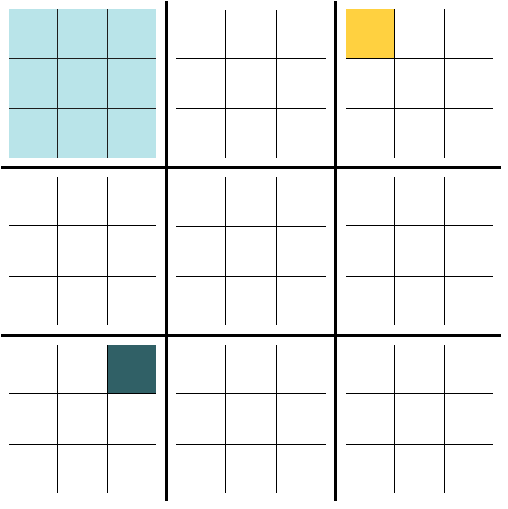
\includegraphics[width=0.6\textwidth]{rule1}
	\captionof{figure}{The yellow player forced the blue player to make his turn somewhere in the light blue marked big tile. The relative position (top-left) of the yellow square on the small board is the same relative position (top-left) as the light blue marked tile on the global board.}
\end{fixedpic}

A victory on a local board is the equivalent to a marked tile on the global board. To win the game, one has to win 3 horizontally, vertically or diagonal aligned tiles of the global board.

If a local board is won or draw, no more moves are allowed there. In case a player was sent to such a board, he is allowed to make his next turn on every other free local board. It's possible that the game ends in a draw, because  no more legal moves are allowed.

\begin{fixedpic}
	\centering
	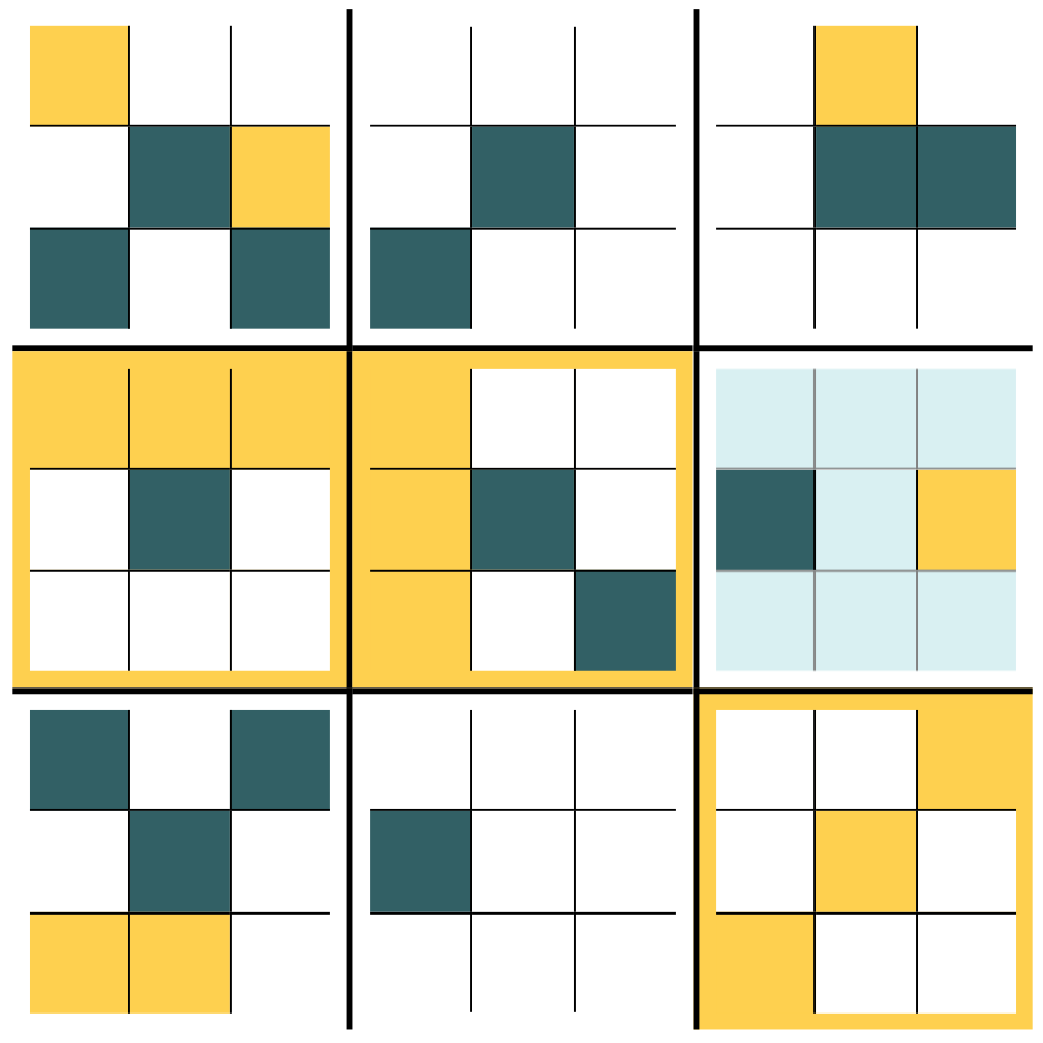
\includegraphics[width=0.6\textwidth]{uttt}
	\captionof{figure}{A random scenario of an Ultimate Tic-Tac-Toe field}
\end{fixedpic}

The yellow marked local fields are already won by the yellow party.

\section{\ac{SLAP} algorithm}



\subsection{\acl{ABP} algorithm} \label{abpalgo}
\begin{fixedpic}
	\centering
	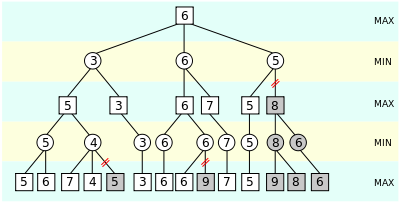
\includegraphics[width=0.9\textwidth]{alphabetatree}
	\captionof{figure}{A representation of an Alpha Beta Pruning tree. \protect \cite{web:aptree} }
\end{fixedpic}



The \ac{ABP} algorithm always starts from one initial game state. This initial game state is represented by the top node. 
%Each game state also corresponded to a value. 
Each game state has a certain number of moves that can be played. For example, when the game starts and the field is empty, there are 81 possible moves that can be played.
All the possible moves are now tried out one after the other. After each move we get a new game state, which also has possible moves again. Even after these moves, we have new game states again. 
%This is how one score after the other is calculated. 
This is how we get all different game states that we evaluate afterwards.
This can be represented as a tree structure. Each node (whether round or square) symbolizes a game state. The branches show the possible moves. Since evaluating all possible game states would be too computationally intensive, a search depth is defined. In the figure the search depth is 4, because four turns were evaluated from the initial node. Now the game states of the lowest row (hands) are evaluated. How this works is in the \autoref{heuristic} described. For now we should know that each game state can be representet by a score. The bigger the number, the better the game state for us. And the better the game state, the sooner we'll win.\\

Now the tree gets evaluated so that in the worst case, the score is as high as possible for us.
That means as much as assuming that the opponent always makes the move that would be worst for us, because a bad game state for us is a good game state for the opponent. 

This is how the evaluation starts at the bottom of the tree. The fourth turn (branches between the last two levels) is played by the opponent (MIN stands for minimizing player, which is equal to our opponent). Therefore, the smallest score is always written in the upper node.\\
\begin{fixedpic}
	\centering
	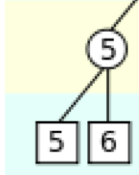
\includegraphics[width=0.15\textwidth]{alphabetabranch}
	\captionof{figure}{Nodes at the bottom left; the smaller value gets written to the upper node}
\end{fixedpic}
The parent node is given the value five, because the minimizing player always chooses the smaller value. This happens with all nodes of this level. The third move is now played by us. We'll take the highest possible score, of course. In this way, the higher-level nodes of the previously filled level are filled with the highest of the possible values. Now it's the turn of the opponent who chooses the worst score for us. The procedure repeats itself up to the initial node. In this way we get the information, which move is best for us. The grey marked nodes and crossed out branches are optimizations of the \ac{ABP} algorithm. So we do not have to evaluate these areas at all and can save computing time.
The search tree gets evaluated after every new turn. In other words, the \ac{ABP} algorithm is able to calculate $n$ turns, which represents the search depth, in advance. Of course, the bigger the search depth $n$ is, the more accurate our moves will turn out. But the deeper the search depth $n$ is, the longer it takes to calculate all moves.

\begin{fixedpic}
	\centering
	
\includegraphics[width=0.9\textwidth]{alphabetalevel}
	\captionof{figure}{All possible game moves in the 3rd level of the search depth, evaluated by the minimizing player}
\end{fixedpic}

The minimal average amount of options per move in the game \ac{UTTT} is five \cite[p.~1-2]{web:amar2013}.
In our case, for simplification purposes, the \ac{ABP} search tree can be pictured with five branches emerging from every new node. With a search depth of $n$, and without the optimizations of the \ac{ABP} algorithm provides, the calculated amounts of all nodes can be calculated with the following equation:  $$a = \sum_{i=1}^{n} 	\delta^{i}$$

\begin{center}
$a$: amount of nodes,
$n$: search depth,
$i$: index,
$\delta$: average move per node
\end{center}


\subsection{Heuristic} \label{heuristic}
The \ac{ABP} algorithm only decides which move is played. But without the heuristic, the \ac{ABP} algorithm would be pointless. The task of the heuristic is to fill the nodes in the \ac{ABP} search tree with meaningful numbers. The more accurate our heuristic will be, the better are the chances for our \ac{SLAP} algorithm to win. The heuristic has only the purpose to evaluate the score of the board, or in other words, calculate a score for each possible \ac{game state}. The better the game state, the higher the score.\\

Now to how the evaluation of the game state works. We award points for certain  \acp{condition} on the board. There are exactly five of these conditions occurring on a board, which are important for our heuristic. The check always takes place in a row, a column or a diagonal. The first two conditions are checked in the small fields.\\


\begin{itemize}
\item One field occupied, two fields empty. The condition occurs three times here. Once in the right column, once in the bottom row and once in the diagonal from top left to bottom right.\\
\begin{fixedpic}
	\centering
	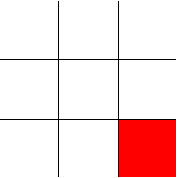
\includegraphics[width=0.2\textwidth]{con1}
	\captionof{figure}{Condition one}
\end{fixedpic}
\item Two fields occupied, one field empty. Here the condition occurs in the lowest row. Note how the first condition occurs three times again, in the left column, diagonally left bottom to the right top and again  middle column.
\begin{fixedpic}
	\centering
	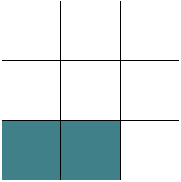
\includegraphics[width=0.2\textwidth]{con2}
	\captionof{figure}{Condition two}
\end{fixedpic}
\end{itemize}
The following three conditions are checked in the large field.
\begin{itemize}
\item One small field won, two small fields not yet determined. Here the condition occurs once in the top row. In this figure, the first two conditions are no longer considered.\\
\begin{fixedpic}
	\centering
	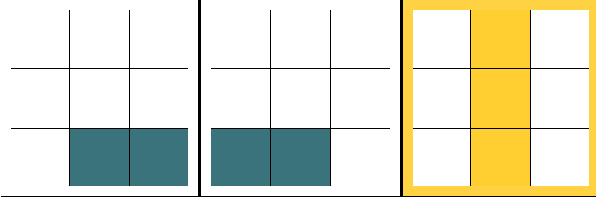
\includegraphics[width=0.6\textwidth]{con3}
	\captionof{figure}{Condition three}
\end{fixedpic}
\item Two small fields won, one small field not yet determined. Here is a visualization of this condition.\\
\begin{fixedpic}
	\centering
	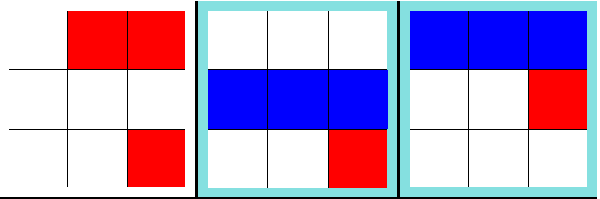
\includegraphics[width=0.6\textwidth]{con4}
	\captionof{figure}{Condition four}
\end{fixedpic}
\item Three small squares won. This also corresponds to a victory. Here the condition occurs in the right column.\\
\begin{fixedpic}
	\centering
	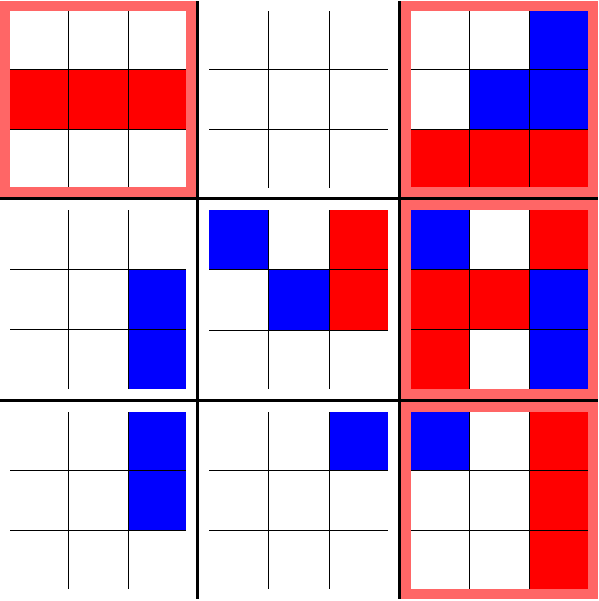
\includegraphics[width=0.6\textwidth]{con5}
	\captionof{figure}{Condition five}
\end{fixedpic}
\end{itemize}
In the following figure, all five occurring conditions are marked with different colors:
\begin{description}
\item[Condition one] Yellow
\item[Condition two] Green
\item[Condition three] Blue
\item[Condition four] Purple
\item[Condition five] Light blue
\end{description}
\begin{fixedpic}
	\centering
	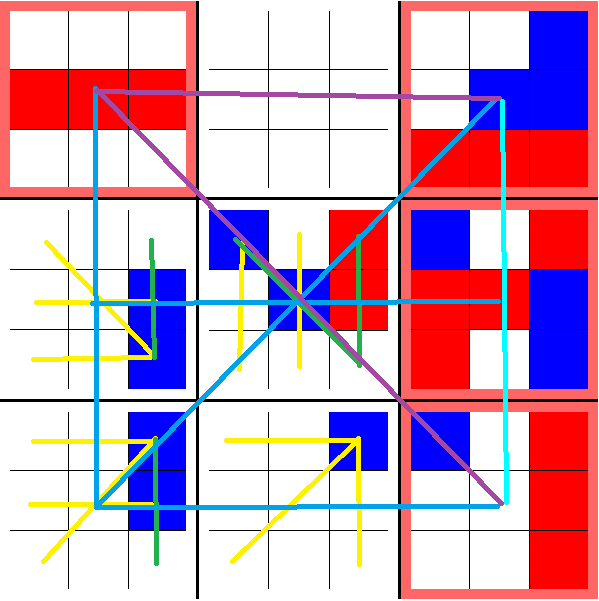
\includegraphics[width=0.6\textwidth]{allcons}
	\captionof{figure}{All Conditions}
\end{fixedpic}
The conditions are determined separately for both players. We take the difference of the conditions of the two players. That is to get a more objective result of the five game conditions. If the difference is $>0$, the first player has better occurring conditions than the second player. If the difference is equal to $0$, both player have the exact same evaluation of the corresponding condition.
If the difference is $<0$, the second player has an advantage with the corresponding condition.


After the subtraction we have five certain numbers, which describe each of the five conditions.  Now, we have to convert them into a meaningful number. This is where the DNA comes into play. The DNA is an object consisting of 5 fields. Each field stands for a factor by which the number, that represent a  condition, is multiplied. Not all conditions should contribute the same value to the final game state evaluation. With the DNA, we are able to control the relative proportions of the five conditions. Let's do a sample calculation using the picture above. Our DNA has the following Numbers.
\begin{center}
\begin{description}
\item[Factor condition one] 1
\item[Factor condition two] 3
\item[Factor condition three] 10
\item[Factor condition four] 30
\item[Factor condition five] 100
\end{description}
\end{center}


In other words, the 5th DNA Value contributes 100 times more value to the final game state evaluation than the 1st DNA factor. The 4th parameter is 10 times more valuable than the 2nd parameter. In the following table, the whole calculation of the value of the game state is shown.

\begin{tabularx}{\textwidth}{|X|X|X|X|X|X|}
\hline
Condition & Occurrence Condition red & Occurrence Condition blue & Difference & DNA factor & Condition Score \\\hline
1	& 0	& 11	& -11	& 1 	& -11 \\\hline
2	& 1	& 3 	& -2	& 3 	& -6 \\\hline
3	& 4	& 0 	& 4 	& 10	& 40 \\\hline
4	& 2	& 0 	& 2 	& 30	& 60 \\\hline
5	& 1	& 0 	& 1 	& 100	& 100 \\\hline
\multicolumn{5}{|c|}{Game state score}&183 \\\hline
\end{tabularx}\\
\\
The effective game state score in this case is 183, which is all the heuristic does.
Based on this information, the Alpha Beta Pruning decides which move to play.



\subsection{Self Learning} \label{selflearning}
To say it in easy terms, the self learning part learns how to estimate the game state in the most meaningful way. It learns which heuristic parameters are important in relation to the other heuristic parameters. In our case, the \ac{DNA}  is responsible for that. The \ac{DNA} dictates, which heuristic parameters are more important and it does that simply with a factor. The \ac{DNA} is also the only thing which changes, while learning.


\subsubsection{Era, generation, organism}
%\subsection{\acp{Era}, \acp{generation} and \acp{organism}}
Let's take a look at how our \ac{SL} algorithm is generated and how it gets better over time.
To get started, we have to create a new \ac{era} and must set up a few things. An era can be compared to several \acp{generation} of humans. 
The era contains all generations. In a human generation, we have several individuals. In our case, we will call our individuals of the generation \acp{organism}. We have to decide, how many organism per generation we want to create. But we have to keep in mind, the more organisms we create, the longer the evolution will take. That's because every organisms will play against every other organisms twice. They play two times, to make sure every organisms has once the possibility to start. It's crucial, that every organism has once the first turn, because from a statistical perspective, the player with the first move wins in 56.17\% of the cases. That is a difference of 12.34\% to the player that starts second, which is a statistically significant advantage \cite[p.~5]{web:tsurel2013}.
The process of playing against each other is called selection. The organisms get rewarded with 3 points when they win, and get 1 point when they end in a draw. When they loose, they won't get any points. The whole process of finding the best organisms of a generation is actually very similar to a football cup.
The amount of games that are played in that way with $n$ participants is $n^2-n$.\\

\subsubsection{Search depth}
We also need to decide the search depth of the alpha beta pruning algorithm the organisms use, while playing against each other. The bigger the search depth, the longer it will take, because the computer has to calculate more scenarios. But the deeper we search, the more accurate results we will get. 
Now after we set up the amount of organisms and the search depth, we can start our new era. The first generation gets created (initialised) with random DNA. The random values are generated between 0 and 2000.
That means the proportion of the different parameters vary vividly. We already know, the organisms with the best random parameter configuration will perform the best. But we don't know yet exactly, which parameters are the most important ones. To find it out, which parameters are the best ones, we now let the organisms play \ac{UTTT} against each other. In other words, we will start the selection. After all matches are finished, we can rank the organisms according to the point distribution system, which we used. The worse half of our first generation will die. And as it is in real evolution, mutation will take place.
The DNA of the better half of the ranking will mutate two times and form a new generation. The best organism of the generation will survive and continue to live in the next generation.
%eventuell genäuere/bessere beschreibung
As described at the beginning, the mutation only affects the DNA. The DNA contains the factor for each parameter and each factor will be mutated with +/- 20\%. This results in an almost totally new set of organisms, which are descenders of the previous generation. The selection starts again for this generation.
This cycle will continue as long as the creator of the era desires to. \\

\begin{fixedpic}
	\centering
	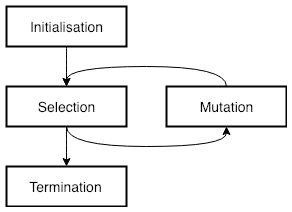
\includegraphics[width=0.4\textwidth]{evoalgo}
	\captionof{figure}{Visualization of an evolutionary algorithm}
\end{fixedpic}


The era which is shown on our website contains 70 generations and each generation consists of 16 organisms.

It took a computer with 3.2GHz and 16 \acp{thread} 8 hours to calculate everything. 14 of 16 threads were utilized. With the following equation, we can calculate the time it took for the computer to play one game:

$$ [t] =  \frac{8h \cdot 60\frac{min}{h} \cdot 60\frac{s}{min}}{16^2 - 16 \cdot 70} = 1.714s$$\\
The average duration of a game between two organisms with above-mentioned computer is 1.714 seconds.

\subsection{Runtime}
Both algorithms, the \ac{SL} algorithm and the \ac{ABP} algorithm, depend on different parameters. These influence the runtime in different ways. If the parameters are too small, we do not get an optimal result. If they are too large, the runtime could be too long.

\subsubsection{Alpha Beta Pruning algorithm}
The \ac{ABP} algorithm has several factors that influence the runtime. One factor is the average search depth, here $\delta$. We cannot influence this factor. The second factor is the search depth, here $n$. The deeper we search, the more games we have to evaluate. So we have a runtime of $\delta^n$ which in the O-notation, which is used in computer science, corresponds to a runtime of $O(N^{m})$. This means that the parameter $n$ influences the runtime exponentially.

\subsubsection{Self Learning algorithm}
The \ac{SL} algorithm has two parameters. One parameter is the number of organisms per generation, $g$ for short. Since all organisms play against each other two times, the formula for the number of games is $g^2 - g$.  The second parameter is the search depth with which the organisms play against each other. We run the \ac{ABP} algorithm once for each move per game with our search depth $n$. Since we don't know the average number of moves per game, we use the variable $\omega$.  And we already know the runtime of the \ac{ABP} algorithm. So in the end we have a runtime of $(g^2 - g) \cdot \omega \cdot \delta^n$. The first part $(g^2 - g) \cdot \omega$, which is influenced by the parameter $g$, has a runtime of $O(N^2)$. The second part, which represents the \ac{ABP} algorithm, is $O(N^m)$ as shown above. This means that the size of the generation affects the runtime quadratically, but the search depth exponentially. Therefore, the search depth of the era must be carefully selected when creating.


\subsubsection{Device Restrictions}
We made our program as device friendly as possible. It isn't required to own a powerful computer to play our \ac{UTTT}, a smartphone is enough. To generate a new era, we got better results with a multicore PC than with a smartphone. That's because the software runs on as many threads as possible, which is the main criteria of fast evolution of an era. 
As we already found out in \autoref{selflearning}, on a computer with 16 threads we needed an average of $[t] = 1,714s$ for one game. If we multiply that by the 14 ($maximal\ number\ threads - 2$) working threads, we get $[t] = 24 s$ per game per thread.
If we now calculate the time for the smartphone we get the following result. $ [t] = \frac{1.5min \cdot 60\frac{s}{min}}{(6^2 - 6)} = 3s$. If we multiply this with the 6 working threads we get $[t] = 3s \cdot 6 = 18s$. This means that one thread of the smartphone actually works faster than one thread of the computer. But in the end, the computer would still be faster because the it has 8 threads more to work with than the smartphone.  Generally spoken, the more threads and speed a device has, the faster the organisms evolve.


%implementation in past
\section{Implementation}
The implementation had two main parts. One part was the implementation of the algorithms and the corresponding one in Dart. The second part was the subsequent integration into the website and the clean design of this.

\subsection{Implementation in Dart}
The implementation in Dart had to be carefully planned. So we started to create the classes that store the data, like the score, for us. This step had to be carefully considered, we then built all the other classes on these classes. Afterwards, of course, we couldn't immediately deal with the algorithms and the actual meaning of the project, but had some milestones, which we could only work through one after the other, because they depended on each other.

\subsubsection{Game Controller}
We already made the classes that store data for us, called modal for short. But to be able to play we needed a lot more information. For example, which moves could be played when a certain game state is active. Therefore we created the \texttt{GameController}, which gives us exactly such information.
\begin{lstlisting}[language=Dart,caption={Structure of the \texttt{GameController}}]
// Returns whether the game is finished or not based on the [state]
bool isGameFinished(GameState state) {
  // Implementation of IsGameFinished
  ...
}

// Return a list of all possible playable moves based on the [state]
List<Move> getAllPossibleMoves(GameState state, [State s]) {
  // Implementation of getAllPossibleMoves
  ...
}

// Reverts a played move on the [state] based on the [revertMove]
GameState revertMove(GameState state, RevertMove revertMove) {
	//Implementation of revertMove
	...
}

// Modifies the [state] based on the [move].
RevertMove playMove(GameState state, Move move) {
	//Implementation of playMove
	...
}
\end{lstlisting}
Since these functions are needed for each individual move, we made these functions as efficient as possible. So we already evaluated every possible Tic-Tac-Toe field and stored it in a cache. If we now evaluate the \ac{UTTT} field, we can access this information and minimize the computing time per call.

\subsubsection{Game}
Because we had all the necessary information for a game state at that point, we could start implementing the game. Therefore we created classes for the game itself and for the players. Since the whole program didn't yet run in the browser but in the console, we didn't implement any input options yet. Instead, we created the simplest algorithm. This algorithm chose a random playable move and played it. So we could let the computers play against each other for the first time. Since the moves were all completely random, the games weren't really exciting. However, it was enough to check that all the rules were followed and that the computer could not play any wrong moves. After that part, we could start with the next milestone.

\begin{lstlisting}[language=Dart,caption={Implementation of the \texttt{RandomMove}}]
class RandomMove extends Algorithm {
  Random r;

  /// Initialises a new Random Algorithm
  RandomMove() {
    r = Random();
  }

  @override
  Move getNextMove(GameState state) {
    List<Move> moves = getAllPossibleMoves(state, State.flip(state.lastMove.state));
    int randomIndex = r.nextInt(moves.length);
    return moves[randomIndex];
  }
}
\end{lstlisting}

\subsubsection{Website}
Because we had a working game so far, we wanted to play it ourselves. That's why we started developing the website. First we had to make sure that the score was displayed correctly. Then we had to create the possibility that when we click into the grid, the correct move is played. After this implementation we were able to play against the computer, but only against the random algorithm. The further implementation of the website is described in more detail in the \autoref{websiteui}. For this milestone we only needed a playable version so that we were able to start implementing the \ac{ABP} algorithm.

\subsubsection{Heuristic}
Before we could start with the \ac{ABP} algorithm, we had to implement the heuristics. The heuristic is used by the Alpha Beta Pruning algorithm. For the heuristic we first created the DNA, the basic component of the evaluation. Based on this DNA, the conditions are then added together. In order to accelerate this evaluation, we already loaded the evaluation for all possible Tic-Tac-Toe fields in the background, as with the game controller. With this information we were able to efficiently evaluate even a large field without much computational effort. This optimization is needed because this function is called by the \ac{ABP} algorithm for every possible game state.

\begin{lstlisting}[language=Dart,caption={Implementation of the heuristic}]
// Returns the evaluated score of the [state] from the
// point of view of the [primaryState]
double evaluateState(GameState state, State primaryState) {
	// Evaluates the score for the [primaryState] and
	// subtract score of the opponent
    return evaluateForState(state, primaryState)
     - evaluateForState(state, State.flip(primaryState));
}

// Returns the evaluated score of the [state] only for the [primaryState]
double evaluateForState(GameState state, State primaryState) {
    double value = 0.0;
    // Checks if the game is finished
    if(cache[state.value][primaryState].three > 0) {
      // Because the game is finished, 
      // only the last parameter of the DNA is relevant
      value += cache[state.value][primaryState].three * dna.bigThree;
    } else {
      // The game is not finished, therefore we analyse all local games
      state.tiles.map((b) => cache[b.value][primaryState]).forEach((info) {
        // If the local board is finished, we don't evaluate the score, because
        // the score will get added in the last step, where we evaluate
        // condition 3 and 4
        if(info.three == 0) {
       	  // Adds the score of condition 1 and 2 for each local board
          value += info.one * dna.smallOne;
          value += info.two * dna.smallTwo;
        }
      });
      // Finally we evaluate condition 3 and 4
      value += cache[state.value][primaryState].one * dna.bigOne;
      value += cache[state.value][primaryState].two * dna.bigTwo;
    }
    return value;
}
\end{lstlisting}

\subsubsection{Alpha Beta Pruning Algorithm}
Now we can describe how we implemented the Alpha Beta Pruning algorithm. Since we already prepared everything, from the heuristics to the game controller, this work was done relatively fast. Since we also built our program cleanly with interfaces, we could simply replace the random algorithm with the Alpha Beta Pruning algorithm and play against it. However, the prerequisite for this was that the heuristic was filled with a meaningful DNA object. We created this by hand, with values that we thought made sense. Afterwards we were able to play against our algorithm. What is striking is that it was already really hard to win against the algorithm, although the parameters were not defined by the computer but by us. That was of course a good sign that our approach could be successful.

\subsubsection{Self Learning Algorithm}
Since our program worked so far, we started with the \ac{SL} part. At first we didn't implement it on the website, but for the console. First we had to create the object that stores the whole process, the era. Then we had to implement the parts described in the \autoref{selflearning} and needed to call them in the correct order. Then we just had to be patient to train a few generations to see if there was any improvement.



\subsubsection{Final Step}
Our main goal was achieved. The algorithm evolved itself and we could play against it. But we didn't want to be satisfied with that yet. That's why we added the self-learning algorithm to the website and added some nice features like color themes and compatibility on all devices. We also kept an eye on the performance and wrote the code as efficient as possible.

\subsection{Website and User Interface} \label{websiteui}
In order that our project is accessible all over the world with different end devices ranging from smartphones to Personal Computers running with different Operating Systems, we thought that it would be the most convenient solution to make a website. 

In general, the static part of the website is made with HTML (Hyper Text Markup Language) and CSS (Cascaded Style Sheets). HTML specifies the structure of a website.  CSS is then required to style everything. The dynamic part, which provides the functionality of the algorithm, was already discussed in the previous subsection. 
Because CSS can be extremely time-consuming, we made use of a CSS Framework called \href{https://materializecss.com/}{Materialize} from Google, which provides cross browser compatible and responsible components such as navbars, buttons, dropdown-lists, cards, modals and many more. To make our website more appealing and fluid, we used CSS animations. For this purpose, we used the website \href{http://animista.net/}{Animista}, which provides ready-to-use CSS animations.

To deploy our website online, we also needed to have a hosting service which offers a server and a domain. Because we already worked with tools of Google like the language Dart and the Materialize Framework, it wasn't far-fetched, that we decided to make use of a hosting provider which also belongs to Google. It's called Firebase. Firebase provides many options for developers such as Real Time Databases or Cloud Messaging, but we only needed to use the hosting opportunity, which supports hosting static files like CSS and HTML.\\

Our website consists of two main parts. The first part, we called it "Reduced View", is mainly designed for an easy game experience, where you can choose between three levels to play against the algorithm. The levels include "easy", "medium" and "hard". Behind the easy level plays the best organism of the first generation. 
The medium level is played by the best organism of the 35th %evtl korrektur
generation and the hard level is the best organism of the whole era. The default search depth of the current game is three. Three is an experiential value, which is the best compromise between search duration and reliability of the algorithm.
The first part of the website contains an explanation of the rules of the game as well.

Via a button in the navigation bar, it's possible to change to a more detailed  part of the website, we called it "Advanced View", which we designed for people who are interested in what's going on behind the scenes. It's possible to see the whole era with all generations and organisms and it's evident, how the algorithm has evolved. It's also possible to generate a new era and calculate everything from scratch. As one plays against a desired Organism, it's also possible to adjust the search depth of the current game dynamically. It's observable, that it takes much longer for the algorithm to make a turn if the search depth is deeper. %evtl zeit erwähnen wie lange es geht

%evtl weglassen oder verbessern
Our Algorithm is separated from the part of the Web, that it is modular and reusable for any other applications like an app or something similar. In programming terms, things are separated with a thing called "Interface". Our Interface in dart is called the Player Interfacer. The Player Interface simply provides the information of our game state and is able to get input from the user interface on our website.

In HTML and CSS, we prepared a 9x9 grid, which we had to fill dynamically with the information of our Player Interface. When the algorithm made his turn, we also implemented a function that shows the player, where he has to play his next turn. 
We also had to make sure, that the calculations of the algorithm didn't run on the same thread as the UI thread of the website. Otherwise, the calculations of our algorithm would block the update of the UI. That would be a bad user experience. In order to prevent that scenario, we made two threads, which allowed the computer to work on both calculations at the same time. 


\section{Progress Evaluation}
As already mentioned, first-generation organisms are produced from randomly generated DNA. Thus, on average, all parameters are still evaluated in approximately the same way. However, this changes over the generations.

\subsection{Expected Result}
According to instinct we can say that condition 5, a victory of the game, should be rated better than condition 1. We can also say that condition 2 should be rated better than condition 1, because with condition 2 we are closer to winning a local game. Also a won local game, condition 3, is better than a nearly won local game, condition 2.
The point is that the conditions are already sorted the way we expect them to be weighted. Condition 1 should have the least weight, condition 5 the most.

\subsection{Received results}
The first generation consists only of randomly created organisms. Nevertheless, a first development can already be observed. The best organism already shows more or less the expected curve. The following conditions are better evaluated than the previous ones. This probably also helped him to victory. Also the last organism is the opposite of the expected result. With the exception of the last parameter, the following conditions are rated worse than the previous ones.\\

\begin{fixedpic}
\centering
\begin{dnadiagram}
\addplot coordinates{(1, 108) (2, 379) (3, 856) (4, 1648) (5, 1745)};
\addplot coordinates{(1, 1408) (2, 1575) (3, 1801) (4, 205) (5, 1508)};
\addplot coordinates{(1, 1586) (2, 790) (3, 494) (4, 439) (5, 697)};
\legend{First of Genration 1,Median of Generation 1,Last of Generation 1}
\end{dnadiagram}
\captionof{figure}{The best, an average and the last DNA of Generation 1}
\end{fixedpic}
While in the first generation only the first organism more or less reproduced the expected curve, in the 5th generation there are already 11 of 16 organisms with such DNA. The remaining 5 organisms show the curve up to the fourth parameter, but the fifth parameter was mutated badly and the curve goes down again. So we have in only five generations already a first trend which plays itself in and already strongly differs from the first generation.
\begin{fixedpic}
\centering
\begin{dnadiagram}
\addplot coordinates{(1, 112) (2, 398) (3, 735) (4, 1410) (5, 1890)};
\addplot coordinates{(1, 122) (2, 362) (3, 750) (4, 1280) (5, 1646)};
\addplot coordinates{(1, 118)(2, 423)(3, 1078)(4, 1507)(5, 1123)};
\legend{First of Genration 5,Median of Generation 5,Last of Generation 5}
\end{dnadiagram}
\captionof{figure}{The best, an average and the last DNA of Generation 5}
\end{fixedpic}
In the tenth generation there is again a conspicuity. Slowly all organisms start to look the same, but condition 3 and 4 stand out. In these organisms, the fourth and fifth parameters are almost identical. Probably because the fourth parameter mutated strongly upwards. Although these organisms do not look like the expected result, they are better than many that look like the expected result. The striking difference to the others is also that the relative difference of condition 3 and 4 is greater than for the others. Precisely because the fourth parameter has probably mutated strongly upwards. According to this observation, the ratio of the parameters plays an important role.

\begin{fixedpic}
\centering
\begin{dnadiagram}
\addplot coordinates{(1, 99) (2, 555) (3, 730) (4, 1294) (5, 2055)};
\addplot coordinates{(1, 60) (2, 324) (3, 642) (4, 1664) (5, 1763)};
\addplot coordinates{(1, 92) (2, 281) (3, 796) (4, 2018) (5, 2055)};
\legend{First of Genration 10,Third of Generation 10,Fourth of Generation 10}
\end{dnadiagram}
\captionof{figure}{Some conspicuous DNA of Generation 10}
\end{fixedpic}

From the tenth generation onwards, these conditions are further developed. So the best of the tenth generation reminds rather of a line, whereas the best of the generation 20 reminds rather of a (half-)parabola. This development continues until generation 70, where we have completed the evolution.

\begin{fixedpic}
\centering
\begin{dnadiagram}
\addplot coordinates{(1, 99) (2, 555) (3, 730) (4, 1294) (5, 2055)};
\addplot coordinates{(1, 103) (2, 369) (3, 1110) (4, 2209) (5, 3033)};
\addplot coordinates{(1 ,74) (2 ,275) (3 ,732) (4 ,1387) (5 ,3976)};
\addplot coordinates{(1, 66) (2, 282) (3, 583) (4, 1451) (5, 5091)};
\addplot coordinates{(1, 61) (2, 327) (3, 717) (4, 1542) (5, 5683)};
\addplot coordinates{(1, 71) (2, 368) (3, 476) (4, 1800) (5, 8907)};
\legend{First of Generation 10,F.o.G. 15,F.o.G. 20, F.o.G. 30, F.o.G. 50, F.o.G. 70}
\end{dnadiagram}
\captionof{figure}{First DNA of different Generations}
\end{fixedpic}

\subsection{Is our algorithm unbeatable?}
The simple answer is no. Even our best organism didn't have a 100\% win rate. So even in his own generation there are organisms which were better or at least could defeat him. And whether we arrive at a point where we reach a 100\% win rate is questionable. During the whole training it never happened that one organism could defeat all the others of the generation. To achieve this, a different approach would have to be tried. One where, for example, more information, such as the current round, influences the heuristics. This would make sense under the assumption that the tactics are different at the beginning of the optimal game than at the end of the game.\\

An other approach which would surely lead to victory, however, certainly exists. But it is not very efficient. This approach would be to set the search depth of our algorithm to 81. 81 for the reason that the game has 81 fields and so even in the worst case the game would be finished after 81 moves. So the algorithm would evaluate every single possible game state. The disadvantage would be the runtime.

The fastest possible victory can be achieved after 17 moves \cite[p.~2]{web:amar2013}. This corresponds to a search depth of 17. The slowest victory would be possible after 81 moves if every square was occupied. So we can make a vague assumption that an average game consists of $\frac{17 + 81}{2} = 49$ moves. With the minimum average move possibility of 5 we have at least $5^{49} = 1.7 \cdot 10^{34}$ in the first move. Optimizing the ABP algorithm would eliminate most of them, but there would still be far too many game states to evaluate.

\section{Challenges}
Errors always creep in during programming. Some are quickly noticed, others remain unnoticed. Of course we also had problems with bugs and unwanted behavior. But only two cases really caused us problems.

\subsection{Worker}
A worker is a feature of web development. You can outsource computational tasks to them so that the main thread, who is responsible for updating the UI, is not under load for too long. Otherwise, the surface is no longer drawn cleanly and the use of the web application no longer feels fluid. Creating such a worker would not have been a problem with JavaScript. But Dart had his pitfalls. Since the programming language is still in development, this feature was not yet implemented cleanly. But we still wanted to use it in order to provide a better user experience.\\
To create a worker, we had to link a JavaScript file, which would get executed in another thread. Our plan was to call a JavaScript file, which afterwards would execute a Dart file, compiled in JavaScript. The problem was that there is not an official way, how we could call a Dart file out of a JavaScript file. We had to look deep in the documentation of the Dart compilers in order to find relevant informations to solve this problems. In the end, the worker worked, even tough it puzzled us many hours.

\subsection{Responsive design with CSS}
When designing a website, it's important to consider, that different end devices are used to visit the website. The screen size and ratio of a normal desktop computer is extremely different from a smartphone. In order to render the website well on all end devices, \ac{responsive} design is required. 

To meet that requirement, fortunately we had the Materialize CSS frame work. Despite that, it wasn't always easy to achieve a seamless design on different end devices. While we developed the website, some components were often displaced, when we accessed the unfinished website with different end devices. 
In the end, even tough it was challenging, we had a well structured responsive design.

\todo{review allenfalls ausführlicher, Edit Damian: Habe noch einzwei sätze hinzugefügt.}
\section{Review}
In retrospect, it was a very interesting project to create. It was very motivating to us, to see the project grow while achieving small goals. Despite the fact that the algorithm works in theory, we had our concerns that it would seamlessly work in a practical implementation. It was a relieve, when we both saw, that the self learning part of the algorithm evolved in accordance to our expectations. Through this project we could also learn a lot. Not only was the programming language new, but also hosting a website, implementing a self-learning algorithm or game. Both of us haven't done that yet.

\subsection{Potential for improvement}
Our algorithm is far from perfect. One point that could be improved is the structure of DNA. Actually, the weighting of a condition is not so important. More important is the difference to the other parameters. Thus, the DNA could have been reduced to four parameters, which would have made training an era faster. Either by giving the first parameter a fixed number instead of mutating, or by describing DNA parameters not as a condition but as a difference to the previous parameter.

Another optimization point would be a variable search depth. Towards the end of the game the possible moves are always minimized. The average number of moves also reduces the number of games to be evaluated, see \autoref{abpalgo}. In order to evaluate the same number of games anyway, the search depth could be increased during the course of the game.
\todo{Zeitformen beachten --> alles in past schreiben}


\clearpage
\listoffigures
\pagebreak
\listoftables
\pagebreak
\bibliographystyle{apacite}
\bibliography{literatur}

%----------------------------------------------------------------------------------------

\end{document}